Recovery and downblending of \gls{HEU} to produce \gls{HALEU} means that 
the fuel contains impurities present in the original
\gls{HEU}. Known impurities in potential \gls{HEU}
supplies to create \gls{HALEU} include $^{232}$U and $^{236}$U
\cite{vaden_isotopic_2018,nelson_foreign_2010},  
which are parasitic neutron absorbers and have the potential to affect 
reactor physics and reactor operation. To investigate the magnitude of this 
effect, this chapter presents models of the use of 
impure \gls{HALEU} fuel in a reactor and compares it to the use of pure 
\gls{HALEU} (only $^{235}$U and $^{238}$U)
to understand how the impurities affect the performance of the reactor.
This chapter of work explores how the fuel affects the reactors, while 
the other chapters explore how the reactors affect the fuel cycle. 

\section{Methodology}
Full core models of the Xe-100 and \gls{MMR} were created in Serpent 
\cite{leppanen_serpent_2014} to model the neutronics and depletion of 
each reactor design. Each model was run using the JEFF 3.12 cross section 
library \cite{koning_status_2011}.

The model for the Xe-100 was obtained from 
\cite{richter_phlox_2021}, an Xe-100-like model that has been used for 
multiple things. The model is available at \cite{richter_zoerichterphlox_2022}
The model was adapted slightly to include control rod systems in the 
graphite moderator. Figure \hl{Xe-100 core figure} shows the axial and 
radial view of the core.

\begin{figure}
    \centering 
    \begin{subfigure}{0.45\textwidth}
        \centering 
        \includegraphics[scale=0.03]{htgr-mr-full-core.inp_geom1.png}
        \caption{Radial view of Xe-100 core model.}
        \label{fig:xe100_core_radial}        
    \end{subfigure}
    \hfill
    \begin{subfigure}{0.45\textwidth}
        \centering 
        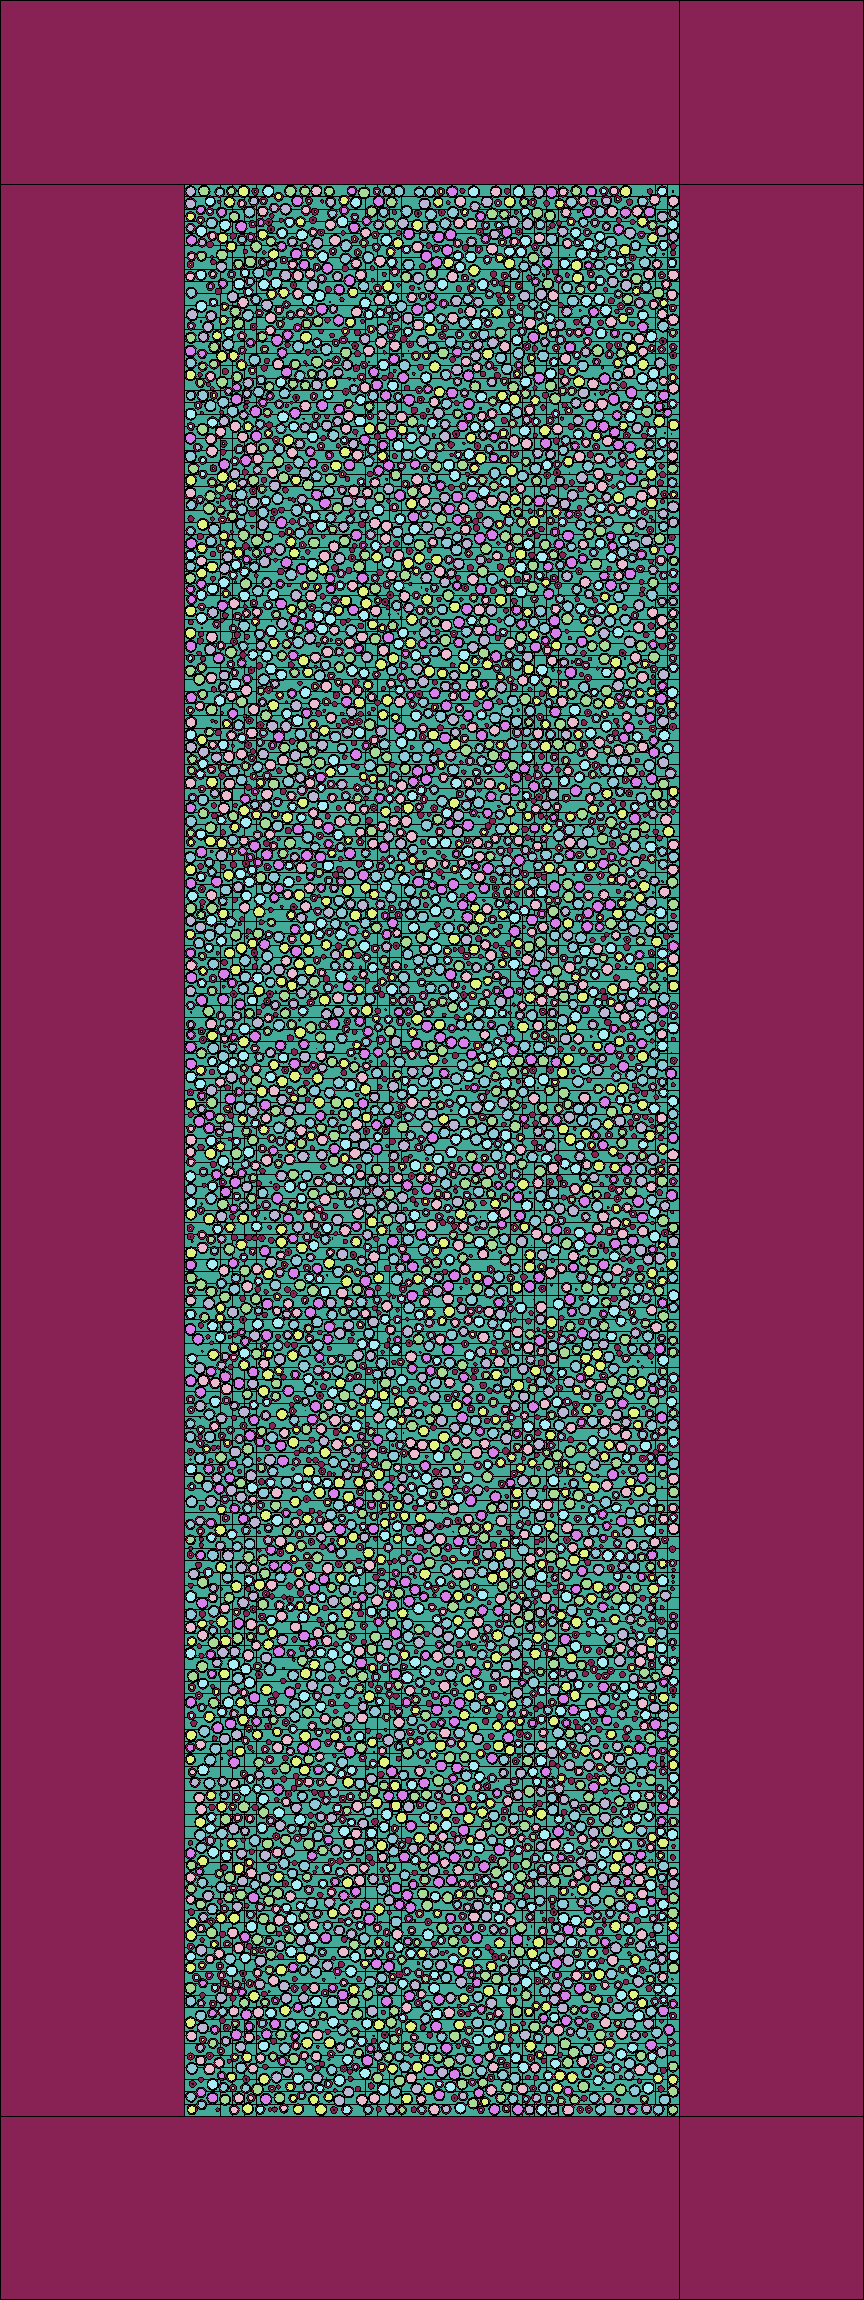
\includegraphics[scale=0.12]{htgr-mr-full-core.inp_geom3.png}
        \caption{Axial view of Xe-100 core model.}
        \label{fig:xe100_core_axial}        
    \end{subfigure}
    \caption{Xe-100 core model made in serpent.}
    \label{fig:xe100_core}
\end{figure}


The \gls{MMR} model was built based on open source information 
about the core design. The model was primarily built based on 
information in \cite{hawari_development_2018}, with adaptations to 
better match published information from \gls{USNC} found in 
\cite{noauthor_usnc_2021}. Figure \ref{fig:mmr_core} shows the radial 
and axial view of the model created. This model was run with XX active 
cycles, YY inactive cycles, and ZZ particles per cycle. The burnup steps
were \hl{figure this out}.

\begin{figure}
    \centering 
    \begin{subfigure}{0.45\textwidth}
        \centering 
        
\includegraphics[scale=0.1]{bachmann-mmr_geom1.png}
        \caption{Radial view of MMR core model.}
        \label{fig:mmr_core_radial}        
    \end{subfigure}
    \hfill
    \begin{subfigure}{0.45\textwidth}
        \centering 
        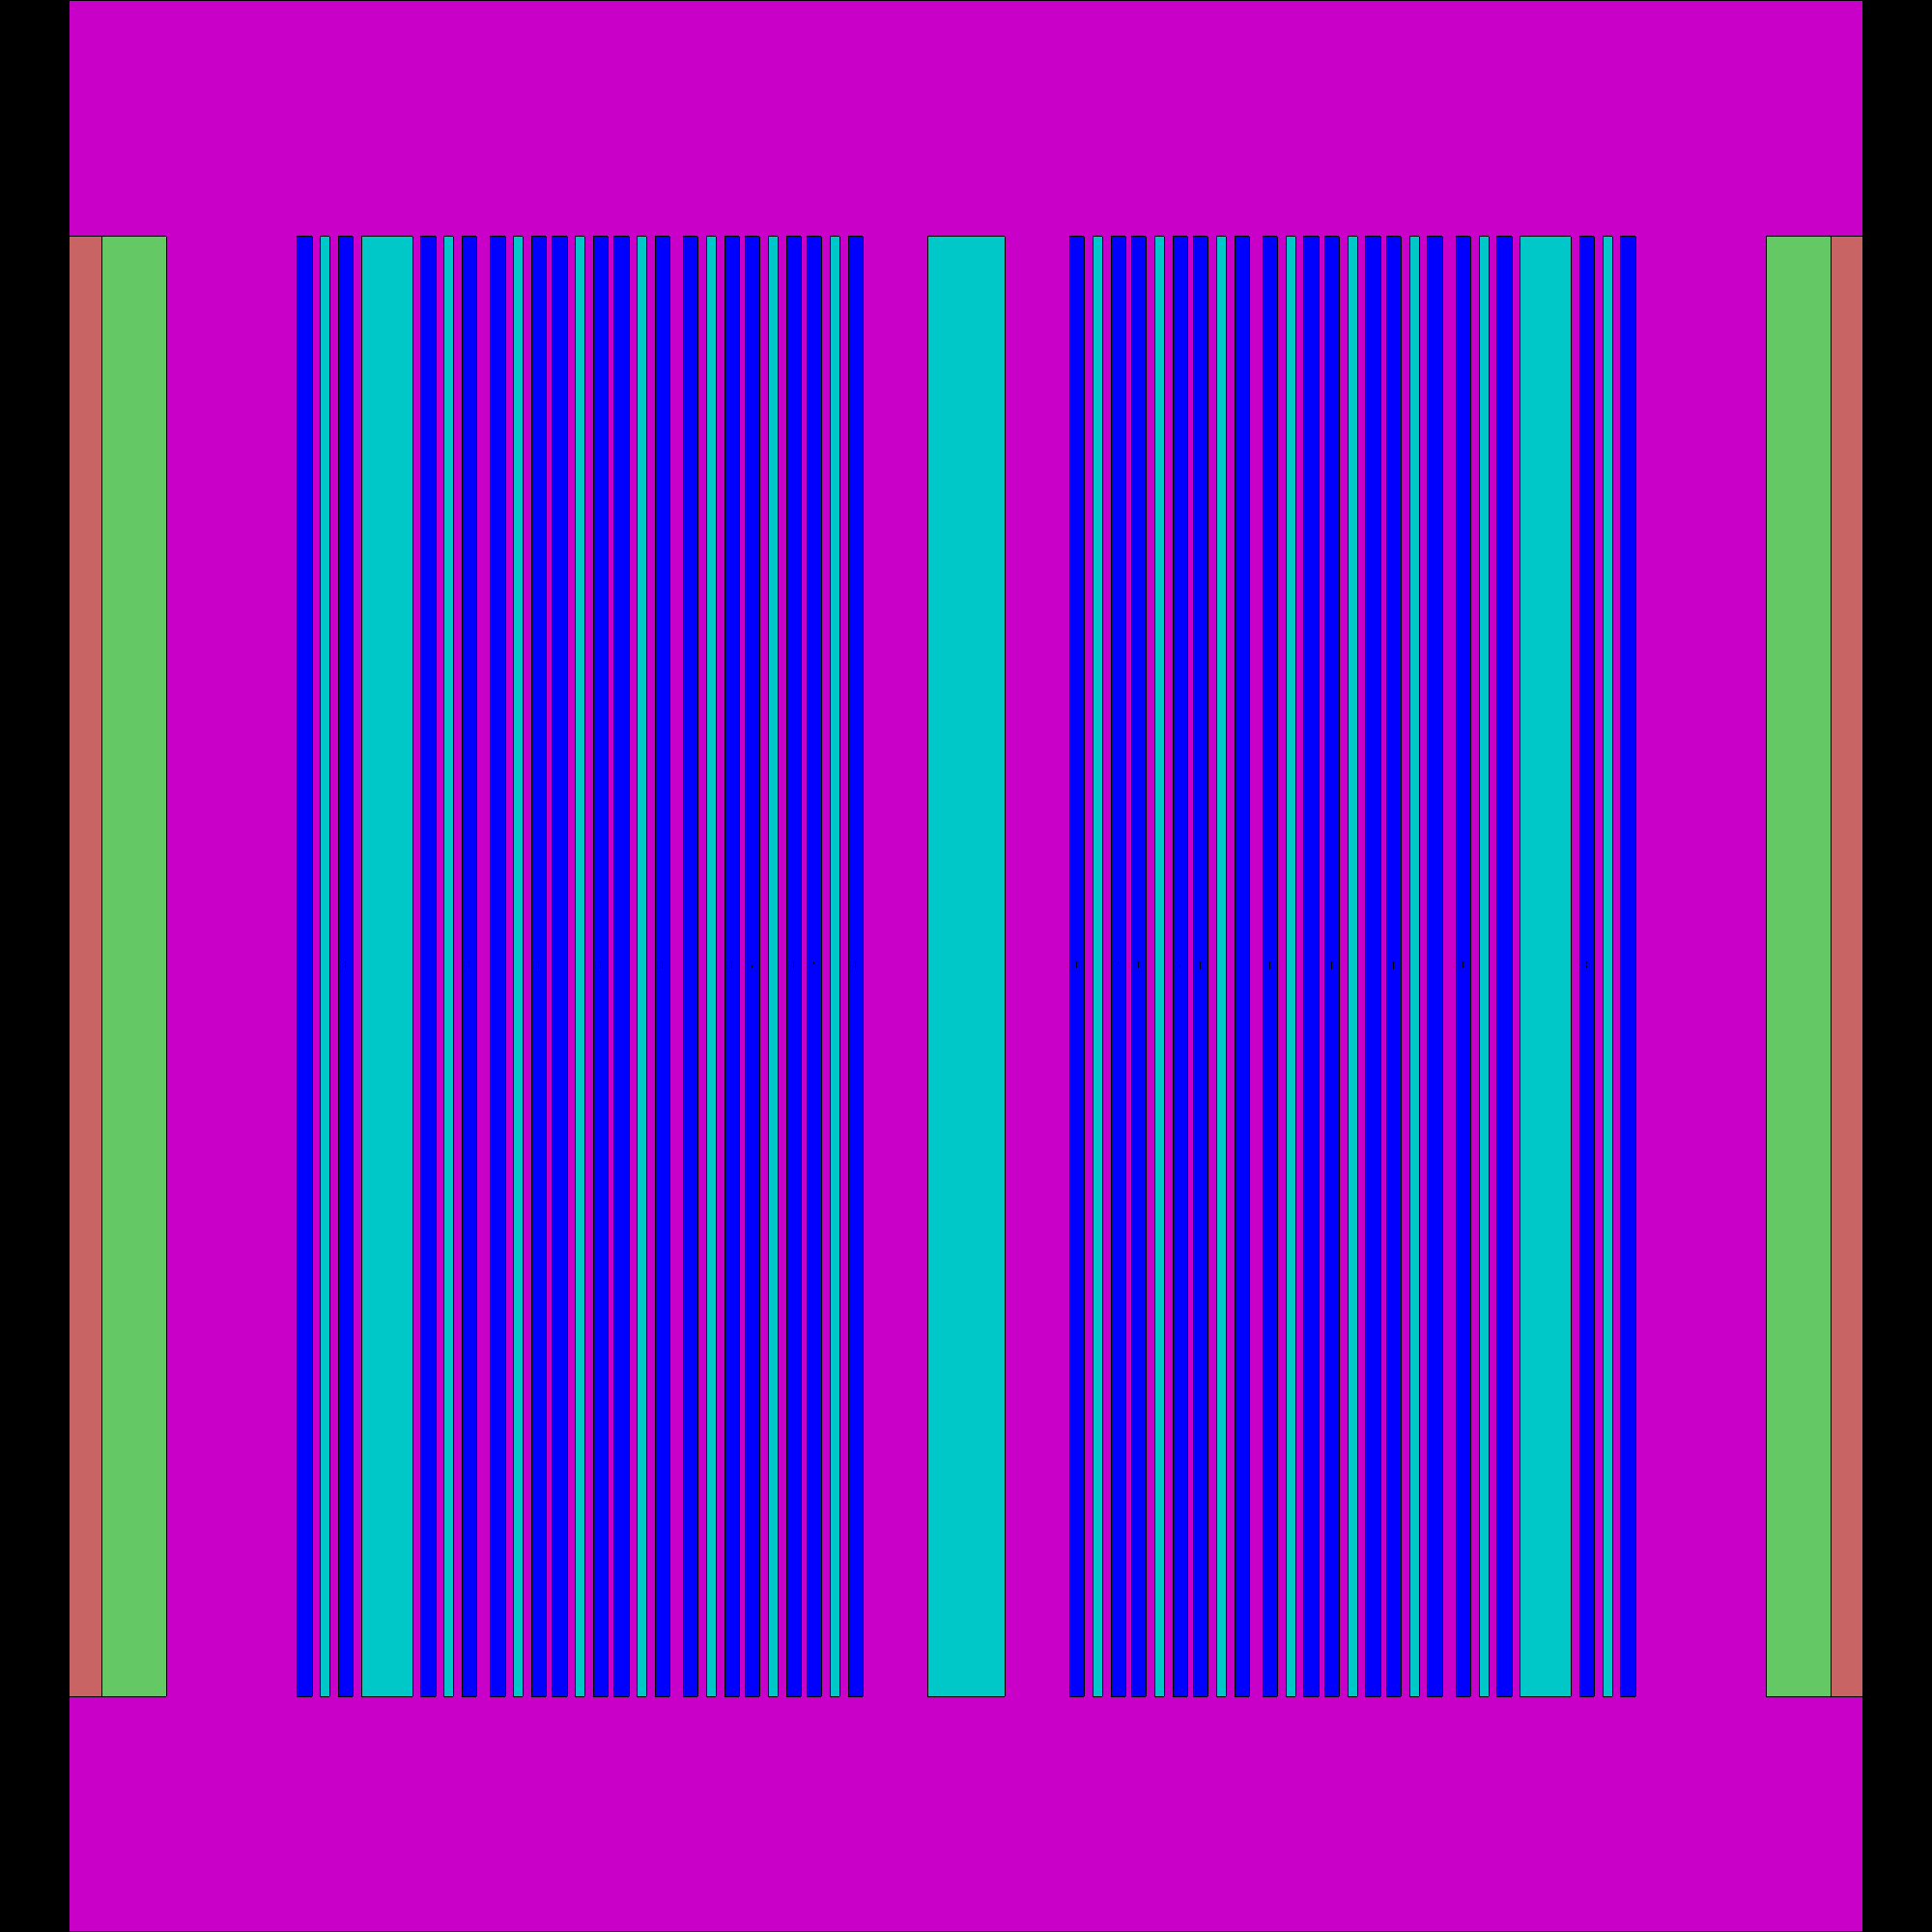
\includegraphics[scale=0.12]{bachmann-mmr_geom3.png}
        \caption{Axial view of MMR core model.}
        \label{fig:mmr_core_axial}        
    \end{subfigure}
    \caption{MMR core model made in serpent. The bright pink is the 
    graphite in the core, light blue is helium cooling channels, 
    dark blue is the FCM. The outer two rings are the 
    beryllium oxide reflector and metal for the RPV.}
    \label{fig:mmr_core}
\end{figure}

 Each burnup step 
used XX active cycles and YY inactive cycles, with ZZ particles per 
cycle. 




The fresh fuel composition for each core was varied to provide 
a comparison of pure and impure fuel.
Material compositions of impure fuel were modeled based on the 
known compositions of \gls{HALEU} from the \gls{EBR} stockpile 
\cite{vaden_isotopic_2018} and the Y-12 stockpile \cite{nelson_foreign_2010}.
Each core was modeled three times: once modeling pure \gls{HALEU}, 
once modeling impure \gls{HALEU} from the \gls{EBR} stockpile, and once 
modeling impure \gls{HALEU} from the Y-12 stockpile.
By modeling the core composition to be entirely composed of impure fuel 
this work reports the most extreme effect that these impurities can 
have on reactor performance. Understanding the limitations of using only 
impure \gls{HALEU} informs on if downblended \gls{HEU} can be used in 
these reactors exclusively for initial reactor core loadings, or if 
infrastructure for enriching natural uranium must be established to 
produce \gls{HALEU} for initial core loadings. 

\section{Results}
Results of each simulation to be compared include the neutron flux at 
\gls{BOL}, mid-cycle, and \gls{EOL}, $k_{eff}$ as a function of burnup, 
fuel temperature reactivity coefficient, and 
$\beta_{eff}$ as a function of burnup. Each parameter provides a 
measurement of the performance of 
the reactor, such as the materials degradation rate, amount of burnable 
poisons required, control rod worth, and the cycle time. Investigating 
each of these results helps to determine if the impurities potentially 
present in \gls{HALEU} will prevent any of the design criteria of the 
reactors from being met. 

\subsection{Xe-100 reactor}

\subsection{MMR reactor}